\documentclass[journal,twoside,web]{ieeecolor}
\usepackage{tmi}
\usepackage{cite}
\usepackage{amsmath,amssymb,amsfonts}
\usepackage{algorithmic}
\usepackage{graphicx}
\usepackage{textcomp}
\usepackage{hyperref}
\usepackage[justification=centering]{caption}
\usepackage{amsmath}
% \usepackage{booktabs}
\def\BibTeX{{\rm B\kern-.05em{\sc i\kern-.025em b}\kern-.08em
    T\kern-.1667em\lower.7ex\hbox{E}\kern-.125emX}}
\markboth{\journalname, VOL. XX, NO. XX, XXXX 2020}
{Author \MakeLowercase{\textit{et al.}}: Preparation of Papers for IEEE TRANSACTIONS ON MEDICAL IMAGING}
\begin{document}
\title{Survey}
\author{
\thanks{This paragraph of the first footnote will contain the date on which
you submitted your paper for review. It will also contain support information,
including sponsor and financial support acknowledgment. For example, 
``This work was supported in part by the U.S. Department of Commerce under Grant BS123456.'' }
\thanks{The next few paragraphs should contain the authors' current affiliations,
including current address and e-mail. For example, F. A. Author is with the
National Institute of Standards and Technology, Boulder, CO 80305 USA (e-mail:author@boulder.nist.gov). }
\thanks{S. B. Author, Jr., was with Rice University, Houston, TX 77005 USA.
He is now with the Department of Physics, Colorado State University,
Fort Collins, CO 80523 USA (e-mail: author@lamar.colostate.edu).}
\thanks{T. C. Author is with the Electrical Engineering Department,
University of Colorado, Boulder, CO 80309 USA, on leave from the National
Research Institute for Metals, Tsukuba, Japan (e-mail: author@nrim.go.jp).}
}

\maketitle

\begin{abstract}
With the increasing application of gigapixel Whole-Slide Images (WSIs) in digital pathology, there has been growing interest in utilizing WSI for survival prediction. This review summarizes and analyzes the recent research on survival prediction using WSI. Firstly, the development and applications of WSI technology, as well as the significance of survival prediction in cancer management, are introduced. Then, different methods for survival prediction are reviewed, including traditional tissue feature analysis, cell-level feature analysis, and deep learning approaches. In tissue feature analysis, researchers predict survival by extracting morphological, textural, and regional features from WSIs. Cell-level feature analysis focuses on the morphological and distributional characteristics of individual cells and computes relationships between cells for more accurate predictions. Deep learning methods, utilizing techniques such as convolutional neural networks and recurrent neural networks, are able to learn complex feature representations from WSIs and achieve high-precision survival prediction. Additionally, the challenges and future directions of WSI-based survival prediction methods are discussed. Overall, utilizing WSI for survival prediction is a promising field that can provide important complementary information for clinical decision-making and personalized treatment.
\end{abstract}

\begin{IEEEkeywords}
% Enter about five key words or phrases in alphabetical order, separated by commas.
Cancer survival analysis,Cancer survival prediction,deep learning,whole slide image
\end{IEEEkeywords}

\section{Introduction}
\label{sec:introduction}
% motivation 添加 

Survival prediction is a direction of statistics for analyzing the duration time that is expected until the events of interest occur,such as the death of the life form of biology.
% 癌症是当前人类面临的最大的健康危机之一,包括各种类型的癌症,乳腺癌,肠胃癌,肺癌等等。临床领域为了减少癌症的危害,可以通过使用wsi类型的切片,由anatomic pathologists使用haematoxylin and eosin (H&E)方法染色的一种组织切片,进行生存预测。生存预测的使用能使得临床医生能够更好地了解患者病情,给出更好的治疗方案,因此能够提高患者的存活率和存活年限。
With the rising importance of precision medicine, the ability to predict patient survival based on individualized characteristics becomes paramount.  WSI, as a rich source of information, offers an unprecedented level of granularity by capturing the heterogeneity within tissue samples. By enabling the high-resolution digitization of entire tissue slides, WSI has not only enhanced the efficiency and accuracy of pathological assessments but has also opened new avenues for predictive modeling and survival analysis.

This review aims to provide a comprehensive overview of the application of WSI in the context of survival prediction. We delve into the intersection of digital pathology and computational methods, exploring how WSI data can be harnessed to predict patient outcomes, especially in the field of oncology.

The introduction of WSI has given researchers and clinicians access to vast repositories of image data, offering new opportunities for feature extraction, machine learning, and deep learning techniques to model and predict patient survival. The ability to analyze tissue morphology, cellular structures, and patterns within whole slide images has the potential to uncover valuable insights into disease progression and prognosis.

In this review, we will examine the key methodologies, challenges, and recent advancements in survival prediction using WSI data. We will also discuss the implications of such predictions on personalized medicine, treatment strategies, and patient care.Additionally, we will explore various aspects of survival prediction using WSI, including the development of novel image features, the utilization of deep learning architectures for image analysis, and the challenges associated with large-scale data management.  We will also consider the ethical and regulatory considerations in implementing such predictive models in clinical practice.

As the fields of digital pathology and computational biology continue to evolve, the integration of WSI into survival analysis represents a promising frontier for improving patient outcomes and advancing our understanding of disease dynamics. This review will serve as a guide for researchers and practitioners interested in leveraging WSI for survival prediction in diverse clinical and research settings.


The complexity of certain data modalities with high dimensionality poses a challenge for physicians in manually interpreting multi-modal biomedical data to decide on treatment and assess prognosis\cite{gevaert2006predicting}. 
The capability to extract "sub-visual" image features from digital pathology slide images—features provides an opportunity for more robust quantitative modeling of disease appearance and potentially improved predictions of disease aggressiveness and patient outcomes\cite{madabhushi2016image}. 

% \section{Background}
% 癌症风险预测是指对潜在的病人的全切片WSI进行分析,也可以结合病人的其他临床数据,例如年龄、性别等,得出病人直至死亡的存活时间。
% 在生存预测问题中,所使用的数据集中,所使用的censorship和survival time基本都是右删失。
In recent years, several computer algorithms for hematoxylin and eosin (H\&E) stained pathology image analysis have been developed to aid pathologists in objective clinical diagnosis and prognosis.
The Cancer Genome Atlas (TCGA) are the most common datasets when discussing the topics of survival prediction.

the observation of one patient is either a survival time $(O_i)$ or a censored time $(C_i).$ If and only if $t_i=\min(O_i,C_i)$ can be observed during the study, the dataset is right-censored [17]. An instance in the survival data is usually represented as $(x_i,t_i,\delta_i)$ where $x_i$ is the feature vector, $t_i$ is the observed time, $\delta_i$ is the indicator which is 1 for a un-censored instance (death occurs during the study) and 0 for a censored instance.

In recent years, the integration of Whole Slide Imaging (WSI) into the realm of survival prediction has emerged as a promising frontier in the fields of digital pathology, oncology, and computational biology. WSI, a revolutionary technology, has transformed the way we analyze tissue samples, providing a comprehensive digital representation of entire pathology slides.

Traditionally, pathological assessments have been reliant on manual inspection and subjective interpretation of glass slides under a microscope. While this approach has served as the gold standard for disease diagnosis and prognosis, it is inherently limited by issues of inter-observer variability, labor intensiveness, and the inability to harness the full potential of the vast data embedded in tissue structures.

The advent of WSI has paved the way for a paradigm shift in tissue analysis. Through high-resolution digitization, WSI generates massive datasets of tissue samples, allowing for a more detailed examination of cellular structures, tissue morphology, and spatial relationships. These digital representations of tissue hold a wealth of information that extends far beyond what can be appreciated by the human eye.

One of the most compelling applications of WSI lies in the realm of survival prediction, particularly in the context of cancer. Cancer remains a leading cause of mortality worldwide, and the ability to predict patient outcomes accurately is paramount for optimizing treatment strategies and improving patient care. With the integration of WSI, researchers and clinicians can extract rich image features and employ advanced machine learning and deep learning techniques to model and predict patient survival.

Survival prediction using WSI offers the potential to uncover subtle patterns, biomarkers, and prognostic factors that may have gone unnoticed in traditional pathology assessments. The granularity and comprehensiveness of WSI data open doors to new avenues of research and personalized medicine, enabling clinicians to tailor treatments to individual patient profiles.

In this review, we delve into the intricate interplay between digital pathology and computational methods, exploring how WSI is being harnessed to predict patient survival. We will examine the methodologies, challenges, ethical considerations, and the implications of these predictions on clinical practice.

As the field of WSI continues to evolve, the fusion of digital pathology and survival prediction holds great promise for advancing our understanding of disease dynamics and ultimately enhancing patient outcomes.

As we delve deeper into this evolving landscape, it is crucial to appreciate the monumental shift brought about by WSI. Its capacity to create digital archives of pathology slides has not only expedited the diagnostic process but has also catapulted computational pathology to the forefront. This dynamic shift, driven by advancements in digital imaging and artificial intelligence, has redefined the scope of pathology by offering a more profound understanding of disease, bolstering diagnostic accuracy, and heralding a new era of prognostic modeling.

WSI's role in survival prediction is particularly significant within the domain of cancer research. It has given rise to the emergence of predictive models that harness the extensive image data contained within tissue samples. By analyzing and extracting pertinent information from these digitized slides, researchers can identify morphological and structural biomarkers, which, when combined with clinical data, offer valuable insights into patient outcomes.

Moreover, the integration of WSI data provides the foundation for the development of prognostic models capable of guiding treatment decisions and improving the overall quality of patient care. The implications extend beyond individualized medicine to population-level studies, ultimately influencing healthcare policy, resource allocation, and public health strategies.

While the potential is immense, it is not without challenges. The management and analysis of vast WSI datasets demand advanced computational infrastructure, robust machine learning algorithms, and a harmonious partnership between pathologists and data scientists. Ethical considerations surrounding patient data privacy, model interpretability, and regulatory compliance also merit attention.

This review embarks on a journey to explore the multifaceted landscape of survival prediction using WSI. It endeavors to survey the methodologies, showcase the milestones achieved, and address the formidable challenges that lie ahead. In doing so, it aspires to serve as a guiding compass for researchers, pathologists, clinicians, and healthcare stakeholders invested in leveraging the symbiotic relationship between digital pathology and survival prediction.

As we advance in this ever-evolving field, the fusion of digital pathology with survival prediction promises to unravel the intricacies of disease dynamics, enhance patient care, and pave the way for a new era of data-driven medicine.

To facilitate future researches on survival prediction, we categorize the models by their methods, as listed in Table \ref{summary table}.
\begin{table}
    \centering
    \begin{tabular}{cccc}
        Category & Method & Highlights & Publication \\
        ROIs   & Data 2   & Data 3   \\
        Features Extraction   & Data 5   & Data 6   \\
        Multimodality   & Data 5   & Data 6   \\
        Graph Neural Network & Data 5   & Data 6
    \end{tabular}
    \caption{Representative Works of Survival Prediction.}
    \label{summary table}
\end{table}

\section{FORMULATION OF SURVIVAL PREDICTION}
\subsection{Survival Analysis}
In traditional survival modeling, it is assumed that the time durations follow an unknown distribution. Among the popular modeling methods, the Cox proportional hazard model stands out, as it focuses on modeling hazards rather than the survival function:
\begin{equation}\label{traditional}
h(t|x)=h_0(t)exp(\beta^Tx)
\end{equation}

The expression involves the time variable $t$, covariates $x$ of dimension $p$ where $x=(x_1,...,x_p)^T$, a vector of regression parameters $\beta=(\beta_1,...,\beta_p)^T$, and the baseline hazard $h_0(t)$. The risk function, denoted as $f(x)=\beta^Tx$, is also referred to as the regression function. The estimation of regression parameters involves minimizing the negative log partial likelihood:
\begin{equation}
    l(\beta) = -\sum_{i=1}^n \delta_i \left( \beta^Tx_i - \log\sum_{j\in R(t_i)} \exp(\beta^Tx_j) \right)
\end{equation}

$n$ represents the patient count, and $t_i$ corresponds to the survival time (censored or observed) for patient $i$, and $\delta_i$ is an indicator variable indicating whether the survival time is censored $(\delta_i=0)$ or observed $(\delta_i=1)$. The term $R(t_i)$ refers to the risk set at time $t_i$, defined as the group of individuals still under study before time $t_i$.

Compared with traditional survival analysis, Katzman et al.\cite{jing2019deep} introduced DeepSurv, a deep fully connected network designed to capture nonlinear relationships between covariates and the risk function. This model replaces the exponential component $\beta^Tx$ in the traditional Cox model's risk function $f(x)$ with a nonlinear deep fully connected network. 

\subsection{Measurement Metrics}
To assess the predictive performances in survival analysis, the ordinary model utilizes the concordance index (C-Index) as the standard evaluation metric, a widely accepted measure for model assessment in survival prediction\cite{steck2007ranking}. 
For a set of Whole Slide Images (WSIs) from $\mathcal{M}$ patients along with their respective labels, the input data is represented as: $$\mathbb{D}_{in}=\{C_1,C_2,...,C_M\},\quad M \geq 2,$$
The C-Index\cite{heagerty2005survival} is expressed as:
% deepconvsurv的
% \begin{equation}
%     C-Index=\frac{\#correctly~ordered~pairs}{\#all~possible~ranking~pairs}
% \end{equation}
% ranksurv的
\begin{equation}\label{c-index-1}
    \mathcal{C}_{index}(\mathbb{D}_{in})=\frac1{\mathcal{M}}\sum_{i:\delta_i=1}\sum_{j:T_i<T_j}\mathcal{I}[(T_i,X_i)<(T_j,X_j)]
\end{equation}

Here, $\mathcal{M}$ is the number of comparable pairs, $T[.]$ denotes the indicator function, and $T$ is the actual observation. 
The C-index ranges from 0 to 1, where a larger C-index indicates better prediction performance, and vice versa. Specifically, 0 represents the worst condition, 1 is the best, and 0.5 is the value for a random guess. 
It is worth noting that the indicator matrix of the C-index has a unique characteristic, as illustrated in the following formulation:
\begin{equation}\label{c-index-2}
    F(X_i, X_j) = 1 - F(X_j, X_i)
\end{equation}
The equation represents the ratio of correctly ordered pairs of subjects' survival times to all possible ranking pairs. 
The Cox proportional hazards model provides a relative risk assessment for a patient compared with others, making the CI a suitable evaluation index.
% 来自Deep Multi-dictionary Learning for Survival Prediction with Multi-zoom Histopathological Whole Slide Images;
% pathomic中有z-score
The Kaplan-Meier curve, illustrating the trend of the survival function $S(t)=\Pr(T>t)$, is employed for assessing the model's effectiveness. 
The survival function adheres to the subsequent relationship at the $k$-th time point (for uncensored samples):
\begin{equation}
S(t_k)=S(t_{k-1})(1-\frac{e_k}{r_k})
\end{equation}

Here, $S(t_{k-1})$ represents survival probability at the time point $t_{k-1}$, $e_k$ is the count of events occurring between $t_{k-1}$ and $t_k$, and $r_k$ is the number of patients with observed time exceeding $t_k$.

To evaluate the survival model intuitively, the entire dataset is stratified into high-risk and low-risk groups using the some risk score quantiles of the predicted relative risk as a threshold. Model performance is assessed by comparing the Kaplan-Meier curves of these groups, with greater separation indicating better performance. The significance of the difference is determined by the $P$ value obtained through the log-rank test, where $P<0.05$ signifies statistical significance.

Survival prediction, a regression problem, involves distinguishing high-hazard and low-hazard patients by adopting a threshold, transforming it into a binary classification task. 
Positive samples include uncensored patients with survival time under the threshold, while negative samples comprise patients with survival/censored time exceeding the threshold. Additionally, the model's performance is evaluated by plotting the Receiver Operating Characteristic (ROC) curve and calculating the Area Under the ROC Curve (AUC).

\subsection{Graph Construction}
%Spectral Graph Convolution. 

Furthermore, it has been widely recognized that the topological properties of instances on pathological images are crucial in medical tasks.Graph is widely employed to represent topological structures.

Generally, let $G=(V,E)$ denote a graph with nodes $V$ and edges $E.$ We define $X\in\mathbb{R}^{N\times F}$ as a feature matrix of $N$ nodes.A in $V$ with $F$-dimensional features, and $A\in\mathbb{R}^{N\times N}$ as the djacency matrix that holds the graph topology. 
Given the graph adjacency matrix A, the graph node embedding X is updated by the message passing function defined in $\mathbf{GCN}$. Consider a multi-layer Graph Convolutional Network (GCN) with the following layer-wise propagation rule\cite{kipf2016semi}:
\begin{equation}\label{GCN-1}
H^{(l+1)}=\sigma\Big(\tilde{D}^{-\frac12}\tilde{A}\tilde{D}^{-\frac12}H^{(l)}W^{(l)}\Big)\:.
\end{equation}

Here, $\tilde{A}=A+I_N$ is the adjacency matrix of the undirected graph $g$ with added self-connections. $I_N$ is the identity matrix, $\tilde{D} _{ii}= \sum _j\tilde{A} _{ij}$ and $W^{( l) }$ is a layer-specific trainable weight matrix. $\sigma(\cdot)$ denotes an activation function, such as the ReLU$( \cdot ) = \max ( 0, \cdot ) .H^{( l) }\in \mathbb{R} ^{N\times D}$ is the matrix of activations in the $l^\mathrm{th}$ layer; $H^{(0)}=X$ . The existing methods for constructing graph on WSI are mainly based on patches and cells.

Graph Construction based on patches: Given a set of sampled patch images $\mathbf{P}=\{\mathbf{P_i}\}$ from WSI, the model has to dump those patches from the margin areas which contains few cells, therefore, the cardinality $\|\mathcal{P}\|$ differs by WSI. Consequently, the graphs to construct for WSIs are of different sizes. Given patches as vertices, vertex features are generated by the different feature extractors


Graph Construction based on cells :For this method, accurate nuclear segmentation is crucial.For already segmented cell nuclei, Pathomic Fusion\cite{chen2020pathomic} use the $K$-Nearest Neighbors (KNN) algorithm and hypothesize that adjacent cells will have the most significant cell-cell interactions and limit the adjacency matrix to $K$ nearest neighbours. Using KNN, adjacency matrix $A$ is defined as: 

if $j\in $KNN$( i) $ and $D(i,j)<d$  otherwise 0


\section{Methodology}
In this section, we review the models of transformer-based models in survival prediction using whole slide images with different methods, including focusing on ROIs, extracting and aggregating image features, combining with other modalities, understanding images with graph neural networks. 
\subsection{Region of Interest}
There exist many methods developed for predicting survival through the information provided by the whole slide images(WSIs).
Rather than utilizing the overall patches from the gigapixel pathology images, the traditional models usually pre-select a subset of critical patches from the region of interest (ROI) as the input data.
Apart from the features extracted from ROIs with the deep neural networks(DNNs), some morphological features of the image patches can be extracted and accessed by the image analysis software named CellProfiler\cite{lamprecht2007cellprofiler}, commonly used for cell phenotypes measurements at that time.
It's the features including cell shape, size, the distribution of pixel intensity in the cells and nuclei and texture of cells and nuclei that the quantitative analysis tool can extract.




\subsubsection{Manually Annotations}
% DeepConvSurv
% To evaluate whether
Taking whole slide images with various size as inputs, in order to do end-to-end survival prediction, DeepConvSurv proposed by \cite{zhu2016deep} randomly chooses the patches among the ROIs annotated by the professional pathologists.
The deep convolutional neural network of DeepConvSurv is shown in fig.\ref{DeepConvSurv}.
\begin{figure}
    \centering
    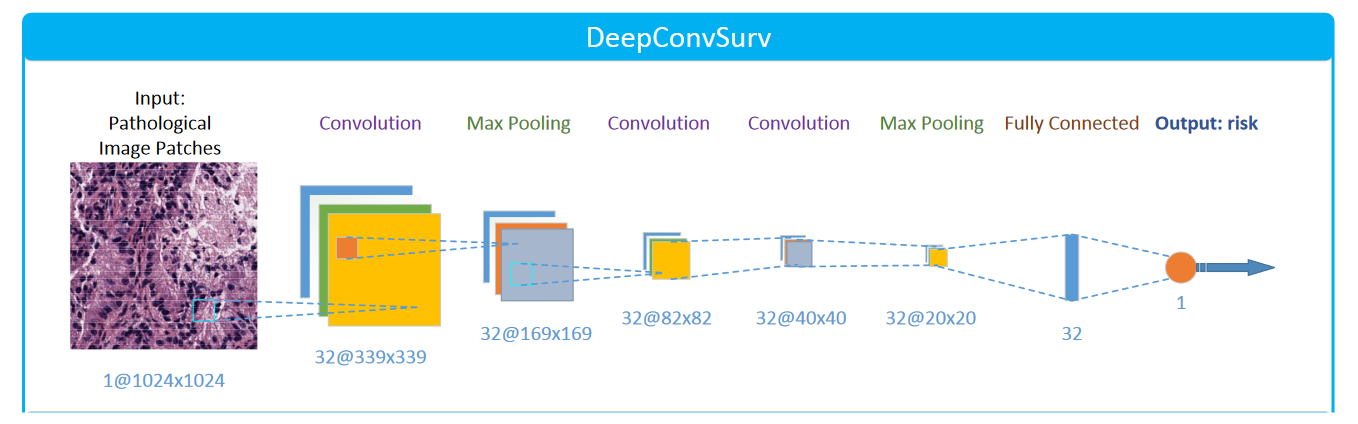
\includegraphics[width=0.8\linewidth]{img/deepconvsurv.png}
    \caption{the framework of DeepConvSurv(image from \cite{zhu2016deep})}
    \label{DeepConvSurv}
\end{figure}
And the experiments showed it could extract more abstract information different from the hand-crafted features generated by the state-of-the-art analysis tool CellProfiler mentioned above.
The primary distinction between the model and the traditional Cox model lies in the exponential component. The loss function for the model is:
\begin{equation}
l(w,b)=-\sum_{i:R_i=1}h_{w,b}^{last}(x_i)+log\sum_{j:t_j>=t_i}exp(h_{w,b}^{last}(x_j)),
\end{equation}

In the equation, $h_{w,b}^{last}(x)$ represents the output of DeepConvSurv, specifically the output of the last layer, where $w$ and $b$ denote the parameters of the network, and $x_i$ and $x_j$ refer to the $i^{th}$ and $j^{th}$ inputs. To simplify, the model will omit the parameters of each layer and express $h_{w,b}^{last}(x)$ as $h^{last}(x)$.
Therefore, the loss function's gradient is changed to:
\begin{equation}
\delta^{last}(x_i)=\frac{\partial l(w,b)}{\partial h^{last}(x_i)}=-1+\frac{exp(h^{last}(x_i))}{\sum_{j:t_j>=t_i}exp(h^{last}(x_j))},
\end{equation}

% Predicting cancer outcomes
% in this paper;results;
With the help of online tool, Mobadersany et al.\cite{mobadersany2018predicting} manually selected the ROIs without tissue-processing artifacts containing overstaining or understaining areas from alternates, which have viable tumor features. 
Faced the difficulty of intratumoral heterogeneity and few availability of labeled data, to obtain better and more robust effects, the model uses the data augmentation techniques and sorted median risks to get prediction results.
And the model eventually gets more accurate outcomes. 
Moreover, the paper provides some publicly accessible datasets with ROIs.

% Pathomic Fusion;microenvironment 
With the assistance of the assembled diagnostic slides offered by \cite{mobadersany2018predicting} with ROIs, characteristics of tumor micro-environment could be got in the built graphs in \cite{chen2020pathomic}.
Because semantic segmentation is executed in ROIs to recognize and localize relevant cells acting as set of nodes in the spatial graph for abstract graph representations.

% convnet [6], [8], [9], [10], [11]
Except this, \cite{zhu2017wsisa}, \cite{di2020ranking}, \cite{yao2020whole}, \cite{abbet2020divide}, \cite{yao2019deep} have shown that random sampling of patches within the tissues in WSIs still makes sense in stratifying phenotypic information which can be improved.

% deepcorrsurv
Not only dose the model in \cite{yao2017deep} use the public cancer survival dataset TCGA, but it also adopts a core sample set from UT MD Anderson Cancer Center during the holistic procedure.
And it takes advantage of the annotations of ROIs to locate the possible tumor regions in pathological images for subsequent steps.

\subsubsection{Sampling Strategy}
% Comprehensive analysis
% In this study;In the NLST dataset;
% esat中提到分类
Some methods adopt sampling strategy to generate candidate patches not limited to ROIs.
Since revealing ROIs requires specialized prior knowledge and expensive labor costs, Wang et al. proposed an automatic model aimed at finding ROIs.
The proposed model in \cite{wang2018comprehensive} can identify tumor regions as ROIs in hematoxylin and eosin (H\&E) stained pathology images using predicted likelihood of image patches, each patch tagged as the highest probability category. 
In this way, some tumor area-related features can be extracted as the descriptors of above ROIs including area, perimeter, convex area, filled area, major axis length, minor axis length and so on.
For the purpose of training the prognostic model indicating that the risk group defined by tumor shape features is an independent prognostic factor, the features are used in the training process.

% capsurv
The model in \cite{mackenzie2022neural} has a automated pipeline excluding the background white space among the identified tissue, then overlooking the sparse cellularity regions and randomly sampling the potential patches from the foreground area.

\subsubsection{Discussion}
In a short, as the methods previously implemented, ROIs routinely ask artificial marking and rigorous reviews to produce passable survival prediction and focusing on ROI ignores the impact of other regions.
Additionally speaking, the ROI-based methods discussed above require pathologists to hand-annotate ROIs, a tedious task.


\subsection{Image Features Processing}
Previous methods often extract image features from patches of whole slide images(WSIs) using the pre-trained model based on the numerous natural images datasets ImageNet theoretically being able to withdraw the low-dimensional features such as edge and texture.However,they have ignored the enormous difference between the WSIs and the natural images.
Recently, some new methods have been proposed to suitably get features from the WSIs to overcome the significant shortcomings.
Without the knowledge of each patch-level labels, the self-supervised learning methods can autonomously impart the outstanding feature extraction ability to the model.
\subsubsection{Pre-trained Image Features Extractor}

% Self supervised contrastive 新方法
The method named SimCLR in \cite{ciga2022self}, one of the self-supervised learning(SSL) methods, using the contrastive learning has excellent feature extraction capacity even comparable to the supervised learning model thanks to the collected 57 digital histopathology datasets with none labels.
% Fine-Tuning and training 新方法
% higt,hgcn直接用;hyper adac,ds-mil用simclr作为策略
Aside from SimCLR as a strategy used in \cite{benkirane2022hyper} and \cite{li2021dual}, KimiaNet from \cite{riasatian2021fine} has also been one of the most welcome pre-trained models used for survival analysis exploiting a variable, multi-organ open image repository lick TCGA, which has been employed directly to extract the feature embeddings of image patches in \cite{guo2023higt} \cite{li2021dual}.

% SeTranSurv;Train Feature Extraction Model;Recent studies have shown;
SeTranSurv, the proposed model in \cite{huang2021integration}(and shown in fig.\ref{SeTranSurv}) applies SimCLR to train the initial feature extraction model ResNet18\cite{he2016deep} to get the specialized model for downstream task survival prediction.
\begin{figure}
    \centering
    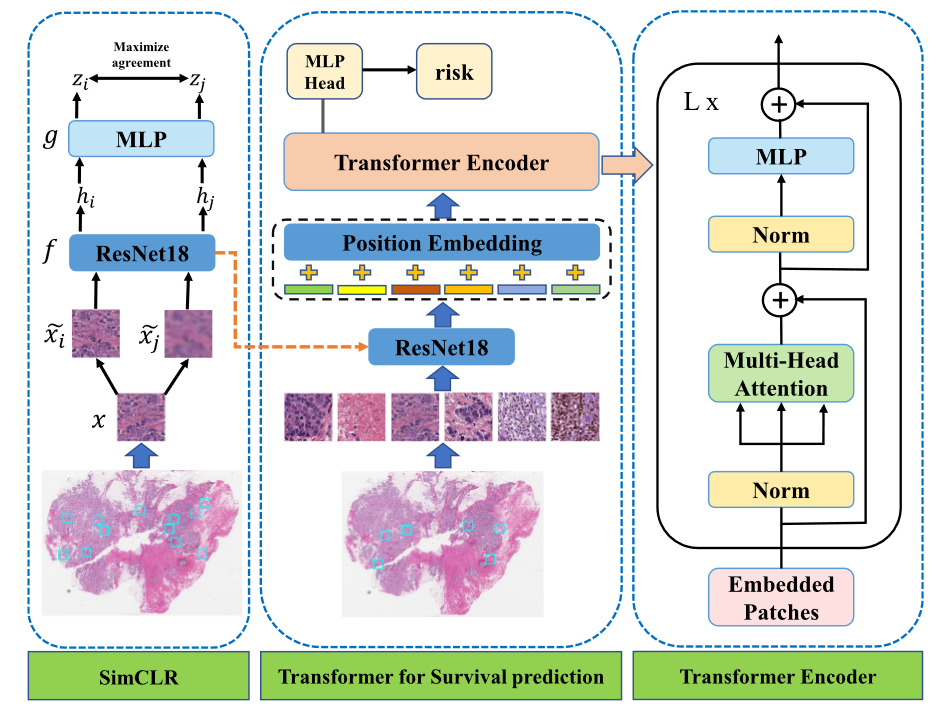
\includegraphics[width=0.8\linewidth]{img/setran.png}
    \caption{the framework of SeTranSurv(image from \cite{huang2021integration})}
    \label{SeTranSurv}
\end{figure}
During the training the model applies the contrastive loss\cite{he2020momentum} to enhance feature extraction ability.
Firstly augmentation module in SeTranSurv using two methods to transform a random image example to a position pair, then the model uses the fine-tuned feature extractor raised above to get the features. 
Considering other images as negative examples ensures that the views of different slide images are far apart in the high-dimensional space and the views of the same image are closer in the process of training.
Additionally, position encodings capturing spatial information and self-attention modules learning correlation between patches are put into the training of the model above to obtain slide-level features and therefore the patient-level features.

The workflow of SimCLR is depicted on the left side of fig.\ref{SeTranSurv}. This consistency is maximized using the contrastive loss\cite{he2020momentum} in the potential space. 
The framework encompasses four major components.
A data augmentation module that randomly transforms any given data instance into two correlated views. 
The image, denoted as $x$ undergoes two different data augmentation methods to produce $\widetilde{x}_i$ and $\widetilde{x}_j,$ forming a position pair.
The goal of the contrastive prediction task is to identify $\widetilde{x}_j$ in $\{\widetilde{x}_k\}_{k\neq i}$ for a given $\widetilde{x}_i$.
A neural network-based encoder $f$ that extracts representation vectors from augmented data instances. 
% ResNet18 is utilized to obtain patch features $h_i=f(\widetilde{x}_i),$ where $h_i$ is the output after the average pooling layer. 
A small MLP $g$ that maps representations to the space where the contrastive loss is applied. 
The MLP is employed to obtain Eq.\ref{SeTranSurv-1}
\begin{equation}\label{SeTranSurv-1}
z_i=g(h_i)=W^{(2)}ReLU(W^{(1)}h_i)
\end{equation}
A contrastive loss function defined for a contrastive prediction task. 
For a given batch size $N,$ the set $\{\widetilde{x}_k\}, k\in\{0...N\}$ comprises a positive pair of examples $\widetilde{x}_i$ and $\widetilde{x}_j$. 

As illustrated on the right side of fig.\ref{SeTranSurv}, the Transformer Encoder\cite{dosovitskiy2020image} comprises multiple encoding blocks, each with constant widths. 
% The dimension $N$ of the encoding block is equivalent to the number of patches sampled from a Whole Slide Image (WSI). 
A learnable embedding is prepended to the sequence of embedded patches $(z_0^0)$ like BERT\cite{devlin2018bert}, and its state at the output of the Transformer encoder $(z_L^0)$ serves as the WSI representation $y$. 
The Transformer encoder consists of alternating layers of multi-headed self-attention (MSA) and MLP blocks (Equations \ref{SeTranSurv-2} and \ref{SeTranSurv-3}).
\begin{equation}\label{SeTranSurv-2}
t_l=MSA(LN(z_{l-1}))+z_{l-1},\quad l=1...L
\end{equation}

\begin{equation}\label{SeTranSurv-3}
{z}_l=MLP(LN(t_l))+t_l,\quad l=1...L
\end{equation}

\begin{equation}\label{SeTranSurv-4}
L(\boldsymbol{R})=\sum_{i\in\{i:S_i=1\}}(-R_i+log\sum_{j\in\{j:T_j\leq T_i\}}exp(R_j))
\end{equation}
% The self-attention module calculates feature correlations between different patches through an attention mechanism. 
Layer normalization (LN) is applied before every block, and residual connections follow every block. 
The MLP comprises two layers with a GELU non-linearity. 
The Transformer Encoder is composed of six encoding blocks, each with four heads, and the hidden size of the MLP is 128.
The resultant $y=LN(z_L^0)$ embodies the amalgamation of high-level semantic features by the Transformer Encoder. 
Passing through an MLP Head module denoted as $R~=$ $W^{(2)}ReLU(W^{(1)}y)$, it directly produces predicted risks. 
The loss function corresponds to the negative Cox log partial likelihood (Eq.\ref{SeTranSurv-4}) designed for censored survival data, where $S_i$ and $T_i$ represent the censoring status and survival time of the $i$-th patient, respectively.

% Cancer Survival Prediction即 convnet
% Feature Extraction Via
Without using convnet-based methods, the model in \cite{fan2022cancer} also considers the self-supervised learning (SSL) methods mainly for making full use of plentiful color information designed for WSI patches or pixels without hand-actuated labels, totally colorization and cross-channel as the pretext tasks.
The colorization model is trained to predict corresponding color channels based on the lightness channel and the letter, on the other hand, is trained to get lightness channel using given color channels data, after which the visualized results indicating highlighted overall structure of nuclei and tissue.

% WSI-HSfeatures 有预训练模型DeepConvSurv
They proposed a survival prediction method \cite{li2023novel} based on tissue pathology and tissue region features extracted from WSIs. 
Use the DeepConvSurv\cite{zhu2016deep} model to extract histopathological features from plaques of actual tissue types (tumors, lymphocytes, stroma, and mucus), and extract tissue region features from the tissue map of WSI by using image processing techniques to locate and quantify tissue regions (tumors, cells, and stroma). 
Firstly, this method uses the DeepConvSurv model to extract the histopathological features of tumors, lymphocytes, stroma, and mucus. 
Secondly, by evaluating the area and proportion of tumors, lymphocytes, and stroma, tissue area features are retrieved from the tissue map. 
Thirdly, Li et al. use the extracted histopathological and tissue regional features to predict patient risk using six survival models.

% PAGE-Net,Pathomic Fusion,PG-TFNet 是特征提取器和多模态结合

\subsubsection{Image Features Fusion}
% EOCSA 没有预训练的模型
In the research of \cite{liu2022eocsa}, Liu et at. introduced the EOCSA framework, which focuses on the survival analysis of EOC by utilizing deep learning techniques to process WSIs. 
They developed a prediction model called DCAS using CBAM\cite{woo2018cbam}, which demonstrated excellent feature extraction capabilities and strong predictive performance. 
The DCAS model employs a cluster-selection strategy to efficiently eliminate redundant information. 
Unlike other deep survival prediction models, they integrated spatial and channel attention modules in the DCAS model to capture tumor-related information. 
Moreover, their weight calculation method enabled the generation of more distinctive patient-level features. 
However, there are still some limitations in the EOCSA framework. 
Firstly, the cluster selection process, while effective in choosing discriminative patches, can be computationally expensive. 
The efficiency of the EOCSA framework may decrease when handling an extremely large number of WSIs. Secondly, not all selected patches are guaranteed to be highly discriminative, which could potentially impact the accuracy of survival analysis if non-discriminative patches are included. 

% SCHMOWDER 没有预训练的模型
In the study of \cite{saillard2020predicting}, two deep-learning algorithms were developed using whole-slide digitized histological slides (whole-slide imaging; WSI) to predict the survival of patients with hepatocellular carcinoma (HCC) who underwent surgical resection. 
The study utilized both a discovery set (Henri Mondor Hospital) for algorithm development and an independent validation set (The Cancer Genome Atlas [TCGA]) for validation. 
Whole-slide images were divided into smaller squares ("tiles"), and features were extracted using a pretrained convolutional neural network. 
The first algorithm, "SCHMOWDER," incorporates an attention mechanism for tumor areas annotated by a pathologist, while the second, "CHOWDER," does not require human expertise.
In the discovery set, both SCHMOWDER and CHOWDER achieved high c-indices for survival prediction surpassing a composite score based on baseline variables. 
These results were further confirmed in the TCGA dataset, where both models outperformed the baseline variables. 
Pathological analysis revealed that specific tumor characteristics, such as vascular spaces, macrotrabecular architectural patterns, and the absence of immune infiltration, were strongly associated with poor survival. 
Overall, this study demonstrated the potential of artificial intelligence in refining HCC prognosis prediction and emphasized the significance of collaboration between pathologists and machine learning for deep-learning algorithm construction that benefited from expert knowledge and contributed to a better biological understanding of their predictions.

% ESAT 没有预训练的特征提取器
In the model of \cite{shen2022explainable}, particularly, a single filter within the convolutional layer is utilized for aggregating one dimension of the multi-dimensional characteristics from neighboring patches. 
The combination of these d filters results in the subsequent layer's feature representations.
Subsequently, following the ViT's procedures, Shen et al. flattened the patch embedding and introduced position embedding. 
In addition, for the purpose of further simplification, they opted for Nystrom-based linear transformers\cite{verma2021beyond} to replace the conventional self-attention transformers. 
The Nystrom approach is applied to approximate the softmax matrix in self-attention by randomly selecting a subset of columns and rows. 
As a result, the time complexity within this module can be reduced.
Moreover, in order to offer understandable rationales for prediction outcomes, they introduced a post-hoc explainability technique for survival analysis.

% deep_survival_analysis 没有预训练的特征提取器,用了不同颜色nlt和rgb的图片
The approach in \cite{liu2022deep} fuses Red, Green, Blue (RGB) color image data with Nucleus, Tumor, Lymphocyte (NTL) data, which includes nuclear segmentation maps, tumor region segmentation maps, and tumor infiltrating lymphocyte (TIL) maps generated through deep learning techniques. 
Essentially, Liu et al. treated the input data as composite images with six channels, incorporating the RGB channels and the NTL channels. 
They adapted a recent state-of-the-art deep learning survival analysis method developed by \cite{wulczyn2020deep} to function with the RGB and NTL channels as well as multi-resolution data. 
The morphological characteristics of nuclei and cells exhibit variations dependent on cancer subtype and stage, making them useful for predictive models. 
Likewise, the spatial properties and distributions of tumor regions serve as important indicators of cancer progression and treatment response. 
In addition to augmenting Whole Slide Images (WSIs) with the TIL, tumor, and nuclear segmentation channels, they trained deep learning models with different resolutions of input data to capture both local and global perspectives on the distribution of TILs, tumor regions, and nuclei in tissue. 

% DSCA 没有预训练的模型
The model DSCA introduced in \cite{liu2023dsca}, inspired by modern feature pyramid networks\cite{wang2021pyramid}, comprises two essential elements: the dual-stream and cross-attention.
The dual-stream module independently processes low- and high-resolution patches, enabling efficient learning of hierarchical WSI representations. 
In the high-resolution stream, a square pooling layer is introduced to drastically reduce the number of high-resolution patches, thereby minimizing computational costs during network training. 
This square pooling operation is implemented using a cross-attention mechanism, where high-resolution patches are pooled under the guidance of a global low-resolution patch. 
This strategy effectively addresses the potential semantic gap between features at different resolutions, promoting seamless fusion of dual-stream features.
The proposed DSCA offers several key contributions. 
Firstly, it introduces a distinctive dual-stream network with cross-attention that fully harnesses image pyramids to enhance the visual representation of WSIs. 
Secondly, the square pooling layer significantly reduces computational costs, serving as a critical component for computational efficiency. 
Lastly, the cross-attention-based pooling method effectively handles the semantic gap between high- and low-resolution features, facilitating improved fusion of dual-stream features and enhancing hierarchical representation for superior prediction performance.

% cellular-level dual-branch global fusion 没有预训练的模型
In the paper\cite{diao2023automated}, Diao et al. introduce a fully automated dual-branch global fusion pipeline at the cellular level to forecast survival based on Whole-Slide Images (WSI). 
In contrast to prognosis methods that focus on nuclei, their pipeline effectively leverages global contextual information, encompassing various cell types and their locations. 
Initially, they generated an embedded WSI map by segmenting and classifying all cell nuclei in the WSI, thereby preserving their spatial information. 
Subsequently, they calculated features separately for the overall WSI and the relationships between different regions within the WSI based on the embedded maps. 
The former features emphasize global cell type and distribution, while the latter features focus on contextual relationships among different or within the same cell types. 
Finally, these two types of global features are fused to evaluate their prognostic implications. 
The proposed method demonstrated higher robustness compared to individual global features. 
Moreover, this comprehensive framework holds potential for predicting survival and treatment responses in other cancer malignancies.


%HVTSurv 没有预训练模型
In this work, Shao et al. proposed a hierarchical visual converter (HVTSurv)\cite{shao2023hvtsurv}for predicting patient horizontal survival, which gradually explores the local horizontal space, WSI horizontal context, and patient level hierarchical interaction in the patient level package. 
For each WSI, the local level interaction layer will first encode the local spatial information. 
Then, spatial mixing is applied to make the model perform similarity calculations on features in different local windows. Finally, all WSI level features will be connected to perform attention pooling, and they use patient level representations to predict the patient's risk of danger. 
It is worth noting that in the local window block, this method adds relative position offset to the self attention calculation and uses Manhattan distance to measure distance, it can make the model more sensitive to short rather than long distances\cite{wu2021rethinking}. 
In the shuffling window block, this method shuffles patient features in different local windows, and then performs window partitioning and self attention calculations.

% KAT 没有预训练模型
They prposed kernel attention Transformer (KAT)\cite{zheng2023kernel} . Compared to ViT \cite{dosovitskiy2020image}, they use cross-attention between the tokens and a set of kernels to replace the token-wise self-attention to achieve information transmission. 
The information flowing in KAT is achieved by cross-attention operation between the kernels and patches, which includes the procedures of information gathering (I.G), information broadcast (I.B), and information aggregation (I.A). 
Through I.G flow, the local information described by the patch representations is reported to their nearby kernels for information gathering. 
Then, through the I.B flow, the regional information summarized by the kernels is broadcast back to the patches. 
Based on the bi-directional message passing flow, communication among the patch representations of the WSI can be accomplished.Finally, through I.A flow ,a classification token is used for summing up the information from all the kernels.
In this information transformation process, they bind a set of anchor points defined by spatial positions in the patch to the kernel of KAT, creating a soft mask based on layered anchor points, guiding cross attention to perceive multi-scale features of WSI.The experiments have demonstrated that the kernel-based cross-attention contributes to a competitive performance for WSI classification and meanwhile significantly reduces the computational complexity of ViT in both the training and the inference stages.

% MHAttnSurv 没有预训练模型
Inspired by the potent multi-head attention mechanism initially introduced in the transformer\cite{jiang2023mhattnsurv} model, the researchers innovatively adapted this mechanism to function efficiently in the realm of multiple instance learning. 
Specifically, the transformer model's core function is to learn context-sensitive representations for every element within an input sequence. 
However, this necessitates attention between every pair of elements, leading to a quadratic increase in computational cost with longer input sequences. 
In the case of the prognostic information extraction task, the sole focus is on the global representation of the input sequence. 
This allowed the elimination of computationally intensive pairwise attentions among the input sequence, retaining only the relevant attentions between global queries and local keys. 
This modification effectively ensures that computational costs scale linearly with input length. 
Building upon this innovation, a multi-head attention framework for cancer survival prediction, named MHAttnSurv, was introduced, designed to work with whole slide images (WSIs) without the need for region-of-interest (ROI) annotations. 
In the MHAttnSurv framework, a backbone ResNet model is employed to extract features from randomly sampled WSI patches. 
These features are subsequently projected into values and keys, which are segmented into several chunks along with a learnable query vector. 
Within each chunk, parallel attention processes work concurrently to pinpoint discriminative regions, and the results from each attention map are concatenated to facilitate survival prediction.

% Surformer 没有预训练模型
This study proposes an innovative MIL neural network termed pattern-perceptive survival transformer (Surformer) for WSI-based survival analysis. 
Briefly, Surformer comprises three components: a ratio-reserved cross-attention module (RRCA), a multi-head selfattention module (MHSA) [24], and a multi-head cross-attention module (MHCA). 
RRCA simultaneously detects global features and multiple pattern-specific local features through a learnable global prototype pglobal and multiple local prototypes plocals and quantifies the patches correlative to each plocals in the form of ratio factors (rfs). 
The ratio information is subsequentially embedded into the feature space for representation enhancement. 

% advmil GAN 对抗性
Inspired by GAN\cite{goodfellow2014generative} and other applications other than image generation\cite{}, the author proposes a new framework for survival analysis of gigabit pixel entire slide images, called Adversarial Multiple Instance Learning (AdvMIL). 
This framework no longer relies on the classical paradigm of event time modeling; On the contrary, it is based on event modeling for adversarial time and integrates multi instance learning required for WSI representation learning. 
The AdvMIL framework is based on event modeling for adversarial time and combined with MIL for WSI representation learning.
The paradigm combining GAN and MIL is implemented through an RLIP (Region Level Instance Projection), which can be used to implement discriminators for WSI survival analysis through fusion networks.

Unlike prior studies that pick and choose specific regions of interest (ROIs) from whole-slide images (WSIs) for survival analysis, new method can utilize the complete tissue and tumor micro-environment without the need for detailed annotations within WSIs. 
Additionally, it can seamlessly incorporate multiple diagnostic slides of various dimensions from a single patient sample for both training and inference in a unified framework.
\subsubsection{Discussion}

\subsection{Multimodal}
One limitation for some existing survival models is that they initially focus on one modality and cannot sufficiently handle multi-modalities data. 
Actually, multi-modalities information could provide complementary and auxiliary information for tumor diagnosis.
For instance, molecular data and whole slide images share relevant representations to describe the same event in tumor growth and symptoms which are very critical for tumor diagnosis.
Therefore,it is essential and necessary to combine and integrate multi-modal data such as pathological images, genotypic information and clinical data for explaining and understanding cancerous heterogeneity and complex symptoms for customized treatments and healings, consequently boosting the survival predictions.
Although hematoxylin and eosin (H\&E)-stained slides are enough to build a comprehensive diagnosis, other modal data can provide a deeper description of the tumor. For example, genomic profiles being comprising of ten thousand dimensional sequences can provide a molecular characterization of the tumor.
Additionally,during the past several decades, multiple clinicians have made clinical cancer survival prediction on the basis of clinical variates and experience, therefore the clinical data is also an important source modality for multi-modal survival prediction.
However, multi-modal survival prediction faces an important challenge due to the huge data heterogeneity gap between WSIs and other modalities, and many proposed approaches use simple multi-modal fusion mechanisms for feature incorporation, which give up mining important multi-modal relationships.
Unlike needle-in-a-haystack challenges, survival outcome prediction involves the modeling of diverse visual elements within the tumor micro-environment. 
These elements are not distinguishable by traditional Multiple Instance Learning (MIL) methods. 
For instance, they include the co-occurrence of tumor cells and lymphocyte infiltrates, which is linked to a positive prognosis. 
This necessitates the modeling of interactions over medium to long distances among instances within Whole Slide Images (WSI).
While it is commonly tackled as a weakly-supervised problem utilizing solely gigapixel Whole Slide Images (WSIs), the conventional perspective on survival outcome prediction views it as a multi-modal learning task.
Due to the variant costs and trauma degree of multi-omics examination, the scenarios of missing modalities are very common.  

\subsubsection{Molecular Data}
% LUNG CANCER SURVIVAL PREDICTION
The model in \cite{zhu2016lung} gets the features from the pathological images extracted using Cellprofiler\cite{lamprecht2007cellprofiler} from the image tiles in ROIs, namely geometry, texture, holistic features.
In addition,the model uses the preprocessed genetic data and one feature selection operation SPACE\cite{peng2009partial} to select representative features to integrate data for the principal component regression model for survival prediction.
The experiments focusing on ADC lung cancer revealed that the results could be better than only using data of genes or images, which demonstrated that the genetic data could actually enhance the prediction performance of the survival analysis model to some extent.

% DeepCorrSurv
Differently, the experiments in \cite{yao2017deep} were conducted on other two cancer types: glioblastoma multiforme (GBM) and lung squamous cell carcinoma (LUSC) using pathological images and molecular data including protein data, Copy number variation(CNV) data and so on. 
But similarly, to fuse the data from different modality for better results, the model firstly learn deep representations from two kinds of data using separate Convolutional Neural Networks (CNNs).Next, the representations passing through the sub-network in the model are connected to get the new representation, which serves as the input of the correlational layer.
Certainly, the deep correlation layer is used to decrease the discrepancy by maximizing the correlation.
After the common layer, the output acts as the input of the survival prediction layer using the negative log partial likelihood as survival loss function.
Compared with the models handling the linear condition, the new model DeepCorrSurv can learn complex correlation using deep neural networks by using the unsupervised method to learn the interactions and the survival loss network to fine-tune the model, eventually getting better results in the comparison experiments about lung and brain cancer.
The results showed that the common representation after maximizing step could bring better performance to the survival prediction measured by the metric named concordance index values or c-index values.

% pnas
In the paper\cite{mobadersany2018predicting}, the model named GSCNN aims for fusing genomic data and second modal data from The Cancer Genome Atlas (TCGA) Lower-Grade Glioma (LGG) and Glioblastoma (GBM) projects. 
If the second modal data are added to the network during the whole training process, the median c index will improve more than simply integrating the second type data into the fully connected layers. Then the model proves that the Molecular subtype is significant in the multi-variable regression model.

% GPMKL
Again, for genomic information, Sun et al. in \cite{sun2018integrating} considered building distinct models to make survival predictions according to the five major molecular subtypes of the breast cancer.
The genomic data chosen in the model consists of gene expression, copy number alteration (CNA), gene methylation and protein expression.
The main idea in the paper is how to merge different types of data as one type, and in this way using multiple kernel learning (MKL) is a choice.
To integrate the genotypic information and image data, GPMKL model was proposed using 5 independent Gaussian kernels and having a integrating step.
The baseline algorithms used that time for comparison includes LASSSO-Cox\cite{tibshirani1997lasso}, elastic-net penalized Cox (EN-Cox)\cite{yang2013cocktail}, Parametric censored regression models (PCRM)\cite{kalbfleisch2011statistical}, Random survival forests (RSF)\cite{ishwaran2008random}, Boosting concordance index (BoostCI)\cite{mayr2014boosting}, Supervised principal components regression (superPC)\cite{bair2006prediction}.
Additionally, two independent models named GMKL and PMKL was constructed only adopting genomic data or pathological images data and four single dimensional models using four types of genomic data were also built. 
Subsequently, the results showed that the gene expression and protein information play relatively more important role than others and CNA makes a little contribution to holistic prediction accuracy.


% OSCCA
One more variation usually ignored is the ordinal relationship among the survival time of different patients, which is assumed independent among patients.
The model proposed in \cite{shao2018ordinal} named OSCCA intends to take advantage of the information.
For extracting features, the model uses the methods in \cite{phoulady2016nucleus} to generate segmented nucleus and get the specific features.
As to gene expression data, the co-expression network analysis algorithms are utilized to derive eigen-gene features.
Considering the correlation between imaging and eigen-gene features, sparse canonical correlation analysis(i.e. SCCA) is used to choose features.
Among the datasets, most patients are censored, denoting that their actual living time is longer than recorded data, while the uncensored patients have the real survival time.
To make full use of the censored state, an ordinal sparse canonical correlation analysis (OSCCA) method is proposed.
In the newly proposed method, the equation estimates the uncensored information, while linear inequalities restrains the ordered relationship between censored and uncensored data. 

% OMMFS
After the model above, Shao et al. developed a new model named OMMFS in \cite{shao2019integrative} using CNV data and level-3 DNA Methylation (DME) data additionally.
The experiments showed that the log-rank test\cite{cheng2017integrative} had better stratification performance than univariate Cox regression method.
Furthermore, the model implements the second feature selection function based on the Generalized Sparse Canonical Correlation Analysis (GSCCA) framework\cite{witten2009extensions} to get the inherent relationship among different modalities.
Likewise the modality in OSCCA, the model under discussing also notices the survival information of patients.
The validation experiments demonstrated that the new model even had superior stratification of early-stage KIRC patients.
To make comparison, the SGSCCA model was proposed with the same objective function without ordered survival information.
However, the feature pre-selection strategy is based on the median value, which is too arbitrary to consider the accurate relevance between features and cancer type.
Also, the image features relies on the regions of interest annotated by pathologists.

% Pathomic Fusion
In the model proposed in \cite{chen2020pathomic}, the cell graphs from histology images are supposed to get the cell-to-cell interactions and cell neighborhood structure.
To build cell graphs, the first step is generating accurate nuclei segmentation, in which a conditional generative adversarial network (cGAN) is used to learn the appropriate loss function for semantic segmentation.
The edge set and adjacency matrix of the graph are constructed using the K-Nearest Neighbors (KNN) algorithm from segmented cell nuclei.
In addition to manually computed statistics, an unsupervised technique called Contrastive Predictive Coding (CPC) is employed to extract 1024-dimensional features from tissue regions centered around each cell.
Graph Convolution Networks (GCNs) learn abstract feature representations for each node by aggregating feature vectors from their neighborhood through message passing.
In scenarios with a high-dimensional feature space and limited training samples, traditional feed-forward neural networks are susceptible to over-fitting. 
To address the challenge and apply more robust regularization techniques when training feed-forward networks on high-dimensional, low-sample-size genomics data, the model adopts normalization layers inspired by Self-Normalizing Networks introduced by Klambaeur et al\cite{klambauer2017self}.
Moreover, the Kronecker Product is used to construct a multi-modal representation. 
The feature vectors of histology images, cell graphs, and genomic features undergo matrix outer product operations to create a multi-modal tensor. 
This tensor captures important interactions among these three modalities in terms of single-modal, bimodal, and tri-modal relationships.
Ultimately, a neural network is trained using fully connected layers with the multi-modal tensor as input. 
The central aim of this method is to fuse heterogeneous modalities with distinct structural dependencies, thereby enhancing research and analysis in cancer pathology. 
To mitigate the impact of noisy uni-modal features during multi-modal training, a gating-based attention mechanism\cite{arevalo2017gated} is introduced to control the expressive power of features within each modality. 
When fusing histology images, cell graphs, and genomic features, the gating mechanism helps reduce the feature space's size before performing the Kronecker Product calculation.

% AMMASurv
To integrate the multi-modality data with different weights, the model proposed in \cite{wang2021ammasurv} uses an asymmetrical Transformer encoder.
The main idea to fuse other modality data unevenly is to add the new nodes and edges into the original graphs.
Different from the normal self-attention in Transformer, the noisy genomic nodes cannot impact the image features because they do not have the outgoing edges, which can only improve themselves by the influence of the imaging features.
% GPDBN
The GPDBN framework in \cite{wang2021gpdbn} comprises an inter-modality bilinear feature encoding module (Inter-BFEM) and two intra-modality bilinear feature encoding modules (Intra-BFEMs) to efficiently handle information interactions both across and within genomic data and pathological images.
This work needs further more data to enhance prognostic performance.

% MCAT
Inspired by methods in Visual Question Answering (VQA), the model in \cite{chen2021multimodal} introduces new approach to let histology patches attend to genes in the survival prediction.
Unlike late fusion-based architectures that simply concatenate WSI-level bag representations with genomic features, the genomic-guided co-attention(GCA) layer captures multi-modal interactions, connecting histology-based visual concepts with gene embeddings, similar to the approach used in VQA.  
These interactions are visualized as attention heatmaps at the WSI level for each genomic embedding.
Additionally, the GCA layer reduces the effective "sequence length" of WSI bags from M instance-level patch features to N gene-guided visual concepts, where N represents the effective sequence length of gene embeddings (with M > N). 
This reduction enables more advanced feature aggregation techniques using self-attention and Transformers, allowing for supervision with entire WSIs, which was previously unattainable.
One limitation of the research was that they utilized a gene set that had been curated previously, and it contained genes with overlapping biological functional impact.

% HFBSurv
To overcome the limitation of Kronecker product, HFBSurv extended GPDBN\cite{wang2021gpdbn} mentioned with the factorized bilinear model.
The model introduces a hierarchical multi-modal fusion approach, which employs factorized bilinear models to progressively integrate information from different levels, reducing computational complexity.  
Genomic data processing involves data cleaning, normalization, and feature selection using randomForestSRC\cite{yu2019breast}.
To process the missing values, the model uses the weighted nearest neighbors algorithm like \cite{ding2016evaluating}.
Pathological images are quantitatively analyzed to extract relevant features. 

% PORPOISE
The main contribution Richard et al. in \cite{chen2022pan} is the development of a research tool, the Pathology-Omics Research Platform for Integrative Survival Estimation (PORPOISE). 
PORPOISE is an interactive platform that provides prognostic markers learned by model for thousands of patients across 14 cancer types. 
It allows users to visualize H\&E images with interpretability overlays, local explanations of molecular features, and global patterns of feature importance. 
They used PORPOISE to analyze high-attention morphological regions in whole slide images and confirmed that the presence of tumor-infiltrating lymphocytes correlates with favorable cancer prognosis, as identified by their model. 
This tool facilitates the discovery of joint image-omic biomarkers.
PORPOISE consists of three network components: an attention-based multiple instance learning network (AMIL) for WSI inputs, a self-normalizing network (SNN) for molecular features, and a multimodal fusion layer (MMF) to integrate feature representations from AMIL and SNN.  
AMIL localizes prognostically relevant regions in WSIs without selective patch sampling and aggregates them for feature representation.  
SNN transforms molecular data into low-dimensional features.  
The model constructs a joint multimodal feature representation for histology and molecular data interactions, which is used for survival analysis.
One drawback of the platform is that while PORPOISE can elucidate "what," it may not always provide an explanation for "why."

% GC-SPLeM
In the model introduced in \cite{xie2022survival}, Xie et al. utilized a multimodal attention module to generate well-structured aggregated feature embeddings for patients and their association matrix. 
Using these embeddings as the foundation, they constructed a graph neural network for predicting survival outcomes.
Thanks to the superior graph quality and effective node aggregation process, the GNN model achieves precise predictions in both datasets with complete and incomplete data, offering a viable solution for handling the problem of missing data.
Each patient is treated as a node in a KNN-affinity graph, enabling the learning and encoding of topological structure and neighborhood information into each patient's feature vector.  
Unlike previous studies that treated patches of WSIs as nodes in a graph, this work innovatively constructs a graph of patients in datasets, motivated by the idea that patients with similar WSI and gene expression data are likely to have similar survival outcomes.  
This approach helps enhance patient representations, especially given the noisy and missing data often present in WSIs and gene expression datasets.

% ponet;pathway-based approaches
Apart from this, another approach to add the genotypic information is using the biological pathway databases to teach the model about the hidden biological functionality.
PONET proposed in \cite{qiu2023deep} uses a sparse biological pathway-informed embedding network for gene expression, additionally adopting the Multi-modal Factorized Bilinear pooling (MFB) method instead of original bilinear model to generate unimodal fusion to catch the modality-specific representations.
Getting each uni-modal fusion, the model can use the output representations as the input of the bimodal and tri-modal fusion respectively utilizing the bimodal attention and tri-modal attention.
Finally the model is trained through the Cox partial likelihood loss proposed by \cite{cheerla2019deep} used for the multi-modalities survival prediction to get the prediction results.

\subsubsection{Clinical Data}
% MultimodalPrognosis
In the model proposed in \cite{cheerla2019deep} named MultimodalPrognosis, clinical, genomic and WSI images data are processed by FC layers, deep highway networks\cite{srivastava2015highway}, the SqueezeNet architecture\cite{iandola2016squeezenet} separately.
The architecture except SqueezeNet is demonstrated in fig.\ref{multimodalprognosis}.
\begin{figure}
    \centering
    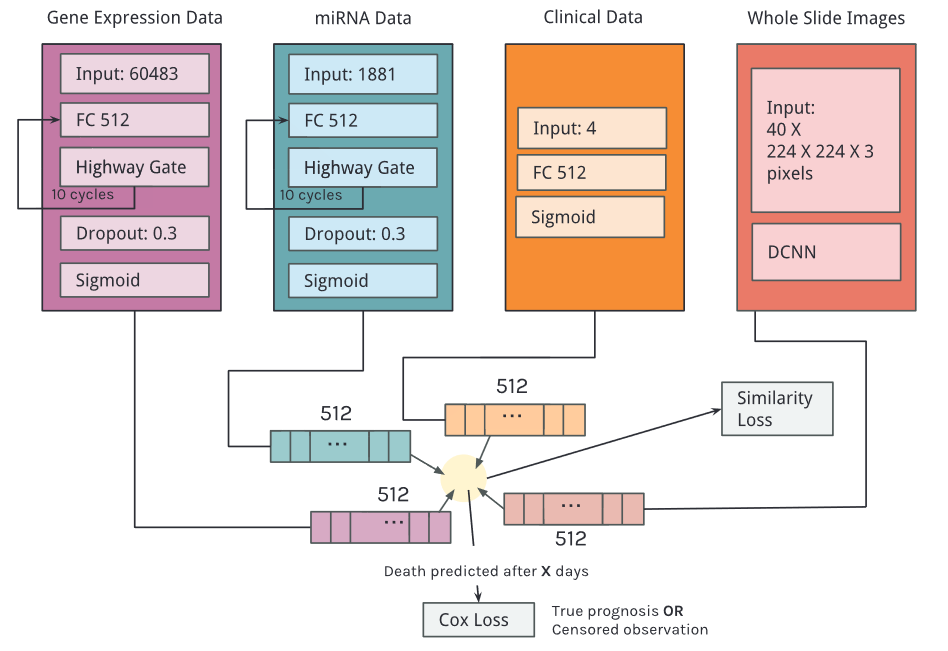
\includegraphics[width=0.8\linewidth]{img/multimodalprognosis.png}
    \caption{the framework of multimodalprognosis(\cite{cheerla2019deep})}
    \label{multimodalprognosis}
\end{figure}
The microRNA data is also passed through deep highway networks discussed. 
One notable problem about the microRNA and clinical data is the missing data.
However, the function of the highway networks dose not stand out without comparison with other methods in the paper.
Then, the similarity loss(Eq.\ref{multimodalprognosis-1}-Eq.\ref{multimodalprognosis-3}) is used to train the model to recognize the patient-distinguishing patterns and correspond the data from different modality to generate associated representations. 
\begin{equation}\label{multimodalprognosis-1}
    sim_0(x,y)=\sum_{i,j\in\mathrm{mod}\text{alities}} \frac { \hat { h }_{0,i}(x_i)\cdot\hat{h}_{0,j}(y_j)}{|\hat{h}_{\theta,i}(x_i)||\hat{h}_{\theta,j}(y_j)|}
\end{equation}

\begin{equation}\label{multimodalprognosis-2}
    L_\theta(x,y)=\max(0,M-sim_0(x,y)+sim_0(x,x))
\end{equation}

\begin{equation}\label{multimodalprognosis-3}
    l_{sim}(\theta)=\sum_{x,y}L_{\theta}(x,y)
\end{equation}
The model aggregates the similarity loss for each pair of modalities that are available.
In the above expression, $x_i$ represents the data for modality $i$, and $h_{\theta i}$ denotes the predictive model for modality $i$. 
It's important to note that the parameter $M$ regulates the 'tightness' of the clustering. 
A higher value of $M$ allows feature vectors for a given patient to be relatively different, as long as they remain similar to a certain extent. 
Conversely, a lower value of $M$ compels feature vectors for a patient to be much closer together, which is generally more desirable but may lead to mode collapse. 
This loss is calculated for every pair of patients in a batch. 
Consequently, the unsupervised model could discern crucial, patient-distinguishing patterns in both genomic and image data. 
Thus, the final loss function is composed of cox loss and similarity loss in the unsupervised model.
The multi-modal dropout was also invented that is dropping whole feature vectors of each modality and accordingly increase the weights of other modalities to build robust representations.
The solution above was then validated in the experiments including visualizing the encodings of the pancancer patient cohort and calculating the C-index values and the results also demonstrated the essence of the adopted modalities.

% PAGE-Net;gpt
This model in \cite{hao2019page} has a two-stage feature extraction process used in a deep learning model for pathology-specific layers. 
In the first stage, a pre-trained convolution neural network (CNN) is used to identify survival-discriminative features in patches of pathological images. 
These features are obtained through dilated convolution layers and max-pooling. 
In the second stage, global survival-discriminative features for a whole slide image (WSI) are generated by aggregating feature scores from multiple patches. 
A two-stage pooling approach, including 3-norm pooling, is used to rank and aggregate the most important features and patches. 
The resulting vector of aggregated survival-discriminative features represents a WSI for a patient, contributing to the integrative deep learning model.
The genome and demography-specific layers in this model are adapted from the Cox-PASNet\cite{hao2018cox}, which is a pathway-based sparse deep neural network. 
The genome-specific layers consist of a gene layer, a pathway layer, and two hidden layers (H1 and H2). 
The gene layer serves as an input layer for gene expression data, with each node representing a gene. 
The pathway layer incorporates prior biological knowledge from databases like KEGG for biological interpretation. 
Connections between the gene layer and pathway layer are established based on biological pathway databases, with pathway nodes representing specific biological pathways. 
The two hidden layers capture nonlinear and hierarchical relationships between the pathways.
Clinical patient data are integrated into the demography-specific layer and combined with genomic features from gene expressions and aggregated survival-discriminative features from pathological images in the final hidden layer of the integrative model. 
To address overfitting in deep learning models with high-dimensional, low-sample-size data, the training technique from Cox-PASNet is applied. 
Instead of training the entire network, small networks are randomly selected, and sparse coding is used to create sparse connections for model interpretability. 
Training continues until convergence, with validation data used to monitor errors and prevent overfitting through early stopping.
PAGE-Net statistically outperformed Cox-EN with histopathological images only and Cox-PASNet with genomic data only. 

% MultiSurv
Similar to \cite{cheerla2019deep}, the model in \cite{vale2021long} can process the missing data including tabular clinical data (herein simply referred to as "clinical"), gene expression ("mRNA"), microRNA expression(miRNA), DNA methylation(DNAm), gene copy number variation(CNV) data and WSI.
If some patients loss the whole modality data, they will be excluded when training the model using uni-modal data.
And the missing data will be replaced by zero matrix when training the multi-modal model.
To avoid over-fitting, the model has the mechanism to select some patients randomly and replace their specific modality data with zero input.
The t-SNE visualization reveals that patients with different cancer types occupy distinct clusters in a two-dimensional space, aligning well with known cancer type prognosis.
The model is trained end-to-end and delivers non-proportional outputs, achieving accurate long-term predictions across various cancer entities. 
Clinical data is identified as the most informative unimodal data modality.

% PG-TFNet
The PG-TFNet proposed in \cite{lv2021pg} comprises three modules: a transformer-based multi-scale pathological feature fusion module, a cross-attention transformer-based multi-modal feature fusion module, and a final Cox layer for clinical data integration. 
The multi-scale feature fusion module processes pathological images at different magnification levels using transformer encoders, capturing relationships between image patches. 
The feature vectors from various magnification levels are concatenated, and a learnable class token and fixed positional encoding vector are introduced to create a multi-scale feature sequence. 
The multi-scale feature sequence is then input into a stack of transformer encoders for multi-scale feature fusion. 
This approach enables the extraction of morphological features at various field-of-view scales, improving the model's ability to understand the relationships between image patches.
The model utilizes a cross-attention transformer module to integrate pathological and genomic data. 
This module combines feature representations from both data types, enabling effective multi-modal data fusion for improved analysis of cancer prognosis.

% DeepCoxSC
This study in \cite{wei2023survival} developed a deep learning-based prognostic model, called MultiDeepCox-SC, for predicting survival outcomes in stomach cancer patients. 
The model integrates histopathological images, clinical data, and gene expression data to improve prognostic accuracy. 
The MultiDeepCox-SC model outperformed the current clinical benchmark model based on pathologic grade, stage, and clinical data, with a higher C-index of 0.744 compared to 0.660. 
It automatedly selects informative patches in histopathological images and identifies genetic and clinical risk factors associated with survival in stomach cancer. 
The risk score generated by the MultiDeepCox-SC model remained an independent predictor of survival outcome even after adjusting for confounding factors. 
The study also validated the model's performance on external datasets. 
The proposed fully automated prognostic tool based on histopathological images, clinical data, and gene expression data has the potential to improve pathologists' efficiency and accuracy and aid clinicians in selecting appropriate therapies. 

% HGCN
The model in \cite{hou2023hybrid} introduces multi-modal graphs as a foundation for a novel Hypergraph Convolution Network (HGCN) designed to extract prognostic-related information. 
The HGCN employs a node message passing mechanism for intra-modal interactions and a hyperedge mixing module for advanced modal interaction. 
Survival predictions were made by combining modalities using an online Multi-view Autoencoder (MAE) proposed in \cite{he2022masked} paradigm during model inference.
The research systematically explored the robustness of the multimodal survival prediction model, addressing an overlooked clinical challenge. 
To handle missing modalities, an online MAE method captures intrinsic dependencies and generates hyperedges. 
Several techniques are employed for handling missing modalities, including zero padding, multimodal factorized method (MFM) for reconstruction, autoencoders \cite{tran2017missing} \cite{liu2021incomplete}, and a lower-bound approach without the online MAE.
The experiments showed that the online MAE module played a key role in improving the prediction robustness.
The study underscored the potential of masked signal modeling for self-supervised learning across different scientific domains.

\subsubsection{Discussion}

\subsection{Graph Neural Network}
The extremely high gigapixel resolution of Whole Slide Images (WSI) requires researchers to divide them into smaller patches for analysis. Most of the previous work has primarily centered around aggregating images based on patches. But based on\cite{levy2020topological}, these methods may also overlook the crucial context between image patches and their neighbors for accurate predictions. Graphs are mathematical models depicting connections between pairs of elements. They are particularly effective for illustrating relationships between individual patches within a Whole Slide Image based on their spatial proximity or correlation. Currently, in risk prediction based on GNN through WSI images, many researchers have also achieved state-of-the-art results.
\subsubsection{Graph Convolution Network}
%DeepGraphSurv
%However, modeling a WSI as graph is not straightforward. Cell-graph [6] is infeasible for WSIs due to its huge number of cells and the many possible noisy nodes (isolated cells). The intermediate patch-wise features are a good option to construct graph with, balancing efficiency and granularity. However, applying CNNs on graphstructured data is still difficult.
DeepGraphSurv\cite{li2018graph} is the first GCN-based survival prediction model that uses WSIs as input. The authors believe that intermediate patch-wise features are a suitable choice for constructing a graph. They integrate global topology features and local patch features of WSIs using spectral convolution operators, which is the core of the entire architecture. In their approach(shown in \ref{DeepGraphSurv}), each patch is treated as a node, and node features are generated using a pre-trained VGG-16 model on ImageNet. The initial WSI graph is built based on patch features, and the VGG-16 feature extractor is not fine-tuned for WSI patches due to the absence of patch labels. Consequently, the initial graph may not accurately represent the topology between WSI patches, which is attributed to the limited training of feature networks.To address this issue, the authors design an independent graph G and  L to describe the topological relationships between specific survival-related WSI patches. This framework can simultaneously learn both local and global representations of Whole Slide Images by integrating local patch features with global topological structures through convolution. Typically, only a few local Regions of Interest (RoIs) in WSIs are relevant to survival analysis. Random sampling may not guarantee that all patches originate from RoIs. The attention mechanism is employed to selectively choose patches by learning their importance. So they introduce a parallel network with attention to adaptively learn attention on node features for selecting more important patches.
\begin{figure}
    \centering
    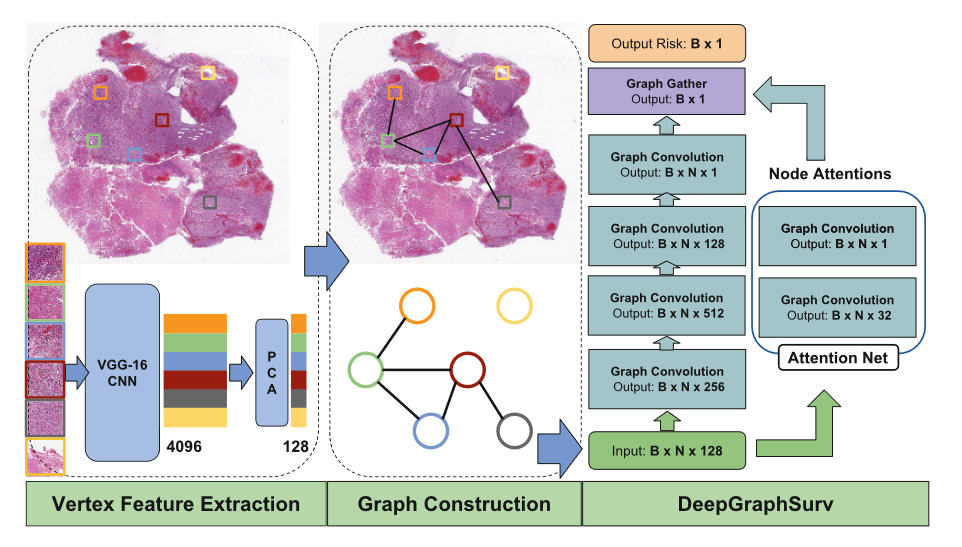
\includegraphics[width=0.8\linewidth]{img/deepgraphsurv.png}
    \caption{the framework of DeepGraphSurv(image from \cite{li2018graph})}
    \label{DeepGraphSurv}
\end{figure}
%Pathomic Fusion
Chen\cite{chen2020pathomic} utilized a Graph Convolutional Network (GCN) approach to extract morphometric cell features from histology images. This article proposes a method called Pathomic Fusion(demonstrated in ref{pathomic}), which is a comprehensive framework for integrating histopathological and genomic features for cancer diagnosis and prognosis. In this approach, cells found within histological tissue are represented as nodes in a graph. These cells are initially identified using a deep learning-based nuclei segmentation algorithm, and connections between cells are established using the K-Nearest Neighbors (KNN) method. The features of each cell are initialized through a combination of handcrafted features and deep features obtained via contrastive predictive coding. The aggregation and combination functions employed in this approach are drawn from the GraphSAGE architecture, with the additional inclusion of node masking and hierarchical pooling strategies from SAGEPool. The primary objective of this method is to extract and learn cell morphological features from histological images.
\begin{figure}
    \centering
    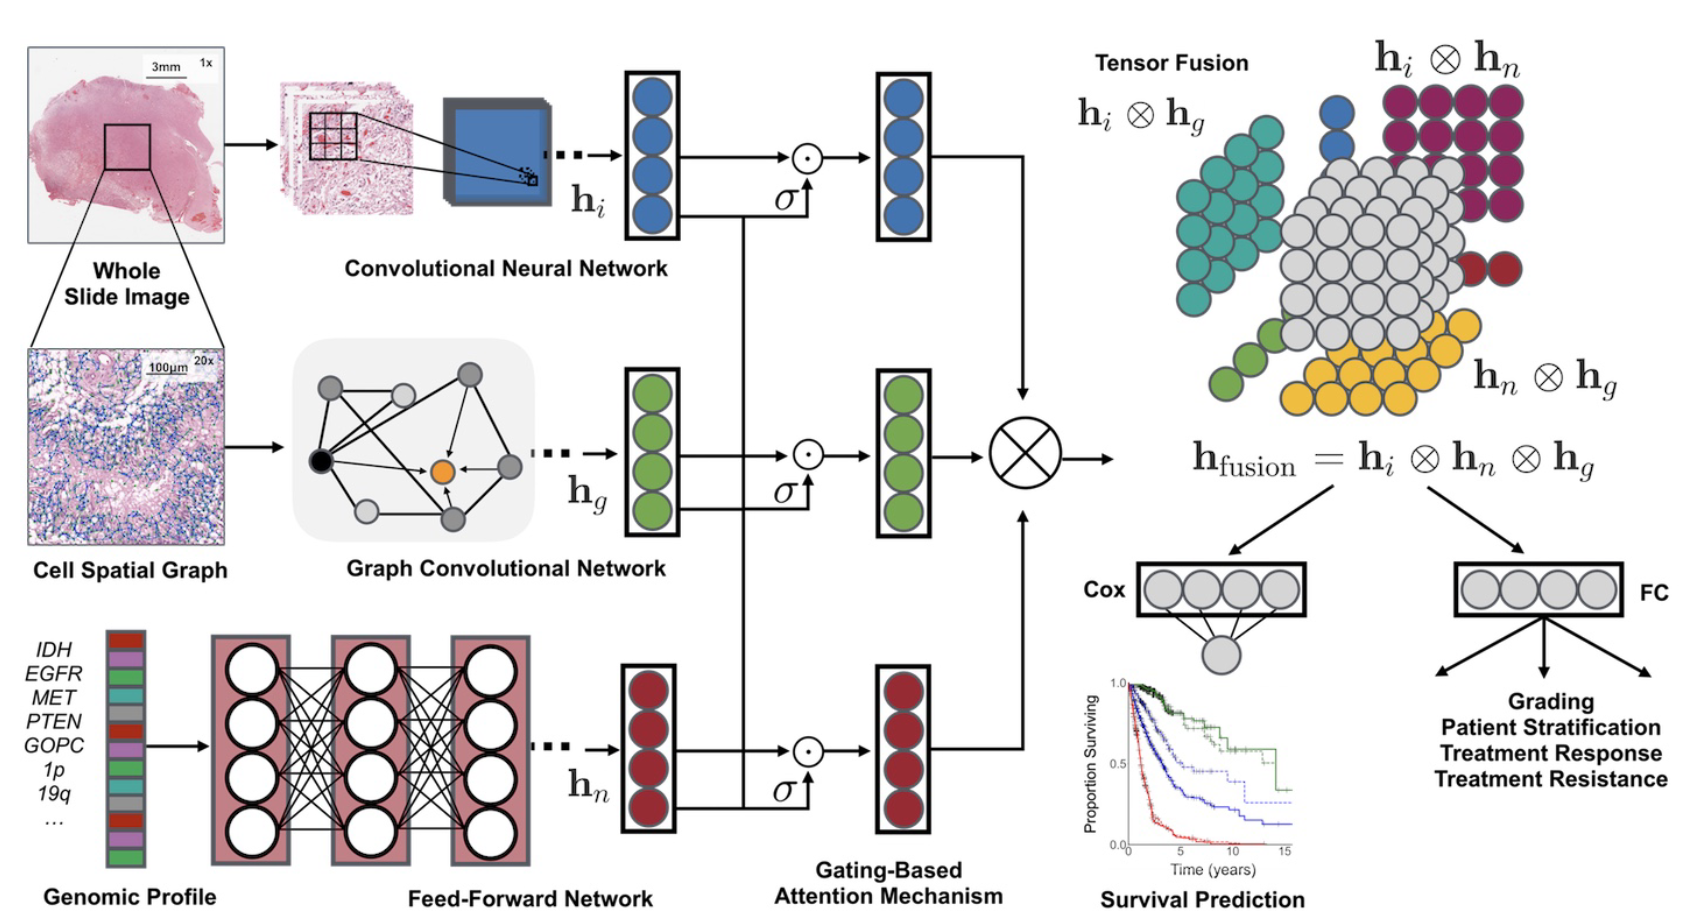
\includegraphics[width=0.8\linewidth]{img/pathomic.png}
    \caption{the framework of Pathomic Fusion\cite{chen2020pathomic}}
    \label{pathomic}
\end{figure}

%Patch-CNN
DeepGraphSurv\cite{li2018graph} proposed sampling patches in a WSI as nodes, followed by constructing edges between patches via feature similarity on the embedding space and using spectral convolutions. 
Alternatively, "Pathomic Fusion" constructed a cell-based graph for small image ROIs followed by spectral convolutions. 
However, in this approach for graph construction, GCNs are unable to learn context-aware features as message passing as feature interactions between adjacent image patches are not modeled.
To enhance the modeling of feature interaction between adjacent image patches during message transmission, Chen et al. \cite{chen2021whole} introduced a context aware, spatially resolved patch based graph convolutional network. This network hierarchically aggregates instance level histological features to capture local and global topological structures in the tumor microenvironment
Their method uses Graph Convolutional Network (GCN), which iteratively aggregates and combines node features of different hidden layers through message passing. The message passing function of the network is adapted from DeepGCN\cite{li2019deepgcns}, including message construction, permutation invariant aggregation, and update functions. Unlike previous graph based methods, they create neighborhoods based on the nearest neighbors in the embedded space, and construct graphs in Euclidean space. This allows them to use spatial convolution to perform local neighborhood aggregation functions similar to convolutional neural networks (CNNs). Compared with other methods of connecting nodes through adjacent image patches, Patch-GCN has improved performance, allowing for learning coarse-grained to fine-grained topological structures in tumor microenvironment.This model is suitable for any weakly supervised learning task in computational pathology that uses slide level or patient level labels, which helps to gain a more comprehensive understanding of representation learning in the tumor microenvironment.


%Survival Prediction for Gastric Cancer via Multimodal Learning of Whole Slide Images and Gene Expression 
%一个基于图神经网络(GNN)的模型来利用患者之间的关联并减轻数据缺失的影响
This paper introduces a gastric cancer survival prediction method called Gc-Splem\cite{xie2022survival}, which employs multi-modal learning by combining whole-slide image (WSI) data and gene expression information. 
The method consists of three key components: the WSI feature extractor, the modal fusion network, and the predictor based on a Graph Neural Network (GNN). 
Firstly, the WSI feature extractor is utilized to extract features from the WSI images. Subsequently, the modal fusion network integrates WSI features with gene expression data to generate high-quality feature embeddings. Lastly, the GNN-based predictor leverages patient associations to make survival predictions, ensuring accuracy through high-quality graph and node aggregation mechanisms, even in the presence of missing data. In a GNN based predictor, there are three key steps: first, construct a K-nearest neighbor (KNN) affinity graph to represent patient relationships, and use cosine distance to connect; Secondly, apply a double-layer graph convolutional network to process patient feature vectors and construct graphs, including element by element multiplication, linear calculation, and ReLU activation function; Thirdly, using the survival prediction layer, similar to the final fully connected layer in modal fusion networks, including the loss function and number of neurons, based on the output of graph convolutional layers for survival prediction.

%TEA-graph 
Attention mechanisms have become almost a de facto standard in many sequence-based tasks.Inspired by it, Petar have presented graph attention networks (GATs)\cite{velickovic2017graph}, novel convolution-style neural networks that operate on graph-structured data, leveraging masked self-attentional layers. Experiments have shown that GAT outperforms traditional graph convolution methods in both direct learning and inductive learning tasks.
The TEA graph\cite{lee2022derivation} adopts a graph attention network (GAT) model structure, which utilizes attention scores in GNN to learn contextual features in heterogeneous tumor environments. Lee et al. adapt the supernode method\cite{stanley2018compressing} to WSI to compress and represent the gigapixel-sized image into memory-efficient graph structures.Using a Graph Attention Network (GAT) to learn contextual features within the tumor environment. It can effectively handle pathological features with varying backgrounds, such as immune cells, and their interactions with the surrounding environment.TEA-graph uses a GAT with positional embeddings to extract the context features around the superpatch by aggregating the neighbourhoods of the superpatch with different attention scores.

%HIGT
In their proposed HIGT framework\cite{guo2023higt}, a WSI pyramid is constructed as a hierarchical graph. Their Hierarchical Interaction GNN and Hierarchical Interaction ViT block have the capability to capture both local and global features. The Bidirectional Interaction module within the latter allows nodes from different levels to interact. Finally, their Fusion block aggregates both coarse-grained and fine-grained features to generate the slide-level prediction.
The paper presents a novel Hierarchical Interaction Graph-Transformer (HIGT) for Whole Slide Image (WSI) analysis, which combines Graph Neural Network and Transformer architectures to learn both short-range local information and long-range global representation of the WSI pyramids.
The HIGT framework abstracts each WSI as a hierarchical graph, where feature embeddings from multi-resolution patches serve as nodes and the edges represent spatial and scaling relationships.
The framework includes hierarchical graph convolution blocks to learn short-range relationships among graph nodes, pooling operations to aggregate local context, a Separable Self-Attention-based Hierarchical Interaction Transformer to learn long-range relationships, and a fusion block to aggregate features from different levels of WSI pyramids for slide-level prediction.
The paper also analyzes the computation cost of the proposed methods and demonstrates that the model maintains promising prediction results while reducing computational cost and model size effectively.

%DeepGCNMIL
However, directly modeling WSI as a graph is computationally complex, and the lack of priori knowledge leads to the difficulty in learning the best graph representation. In WU’s research, a multi-instance learning (MIL) framework called DeepGCNMIL\cite{wu2022deepgcnmil}was introduced for survival analysis of gigapixel Whole-Slide Images (WSIs). Initially, the ResNet50 pretrained model from ImageNet was employed to extract the morphological features of patches, which were subsequently clustered using the K-Means method. Within the context of a graph structure, a Graph Neural Network (GNN) was applied, treating each feature patch in every cluster as a node. The GNN subnetworks were embedded into a deep learning architecture, consisting of three layers of Graph Convolutional Neural Networks paired with ReLU activation functions, and a final addition of global pooling layers, such as average pooling. Relationships between feature patches were established through edge connections between nodes, and feature information was forwarded to generate the entire graph's feature vector. This approach effectively modeled relationships between patches, extracting meaningful representations of phenotypes for survival prediction. Finally, multiple heads and aggregated phenotype features were introduced to the WSI representation, facilitating prognostic risk assessment. It is more suitable for situations where manual ROI labeling is lacking in large-scale cancer datasets, and can simultaneously process prognosis predictions for cancer patients with different numbers and sizes of entire slide images. Moreover, this model can be easily transplanted to other cancer datasets and applied to other tumor types.

%GraphLSurv: A scalable survival prediction network with adaptive and sparse structure learning for histopathological whole-slide images
The paper\cite{liu2023graphlsurv} presents a structural learning approach aimed at capturing potential patch correlations and generating adaptive and sparse structures. This approach allows for optimal patch selection for feature aggregation and efficient GCN training, eliminating the need for predefined, fixed graphs tailored to the task.The proposed method introduces a scalable graph convolutional network called GraphLSurv designed for survival prediction based on gigabit-pixel full-slide images (WSI). This framework comprises three key components: WSI preprocessing, survival perception structure learning, and GCN-based survival prediction.In a broader context, the author conducts a review of deep learning methods relevant to gigabit-pixel WSIs, categorizing them into two groups: graph-based and graph-free approaches. GraphLSurv stands out by generating adaptive and sparse structures for patches, allowing it to dynamically capture and adjust potential patch correlations.

%GraphLSurv: A scalable survival prediction network with adaptive and sparse structure learning for histopathological whole-slide images
Given the problems posed by pre-fixed or densely-connected patch structures,this paper\cite{liu2023graphlsurv} proposes a structure learning method to construct adaptive and sparse patch correlations. A simple way to construct a patch structure is to connect each patch with its k nearest neighbors (k-NN) or adjacencies. This article proposes a structural learning strategy to generate adaptive and sparse structures, using a patch similarity learning technique that can optimize connection patches and directly calculate edge connectivity without relying on previous computational models used in DeepGraphSurv. This method can be summarized as calculating the cosine distance for each patch to measure patch similarity. This outputs a symmetric matrix, where the size of each element represents the strength of the edge connection. Afterwards, if the connection strength of AL is less than the threshold (x), they mask its elements to 0. This operation produces a sparse structure that can filter unnecessary connections, thereby reducing noise correlation in AL.

%H2-MIL: Exploring Hierarchical Representation with Heterogeneous Multiple Instance Learning for Whole Slide Image Analysis

This article proposes a new multi instance learning framework H2-MIL\cite{hou2022h} for full slide image  analysis based on graphical neural networks. It utilizes heterogeneous graphics of different resolutions to simulate the characteristics and spatial scale relationships of multi resolution patches. Firstly, use heterogeneous graphs with resolution attributes to represent WSI with multiple resolution levels. Then input it into the H2MIL network, which consists of multiple RAConv modules and IHPool modules, forming the core of the network. This part constitutes the learning process of graph attention convolutional networks, where nodes continuously aggregate information from their neighbors to extract dense but differentiated feature representations. This helps to mine hierarchical semantic information for WSI analysis. Finally, based on the learned representation, a WSI level classifier is used for prediction. This framework includes a resolution aware attention convolution (raconV) module for learning compact discriminative representations from graphs and addressing the heterogeneity of node neighbors at different resolutions. It also integrates the Iterative Hierarchy Pooling (IH Pooling) module, which can gradually aggregate heterogeneous graphs based on the scaling relationships of different nodes, thereby exploring structured information related to WSI and tasks.

%SlideGraph+: Whole Slide Image Level Graphs to Predict HER2 Status in Breast Cancer
The author proposes a new graph neural network (GNN) based model, called SlideGraph+\cite{lu2022slidegraph+} for directly predicting HER2 state from full slide images of conventional hematoxylin and Eosin (H\&E) glass slides. This model captures the overall organization and structure of an organization, unlike traditional patch based methods with limited visual context, which can manipulate graphics at the entire slide level. The framework proposed by this network consists of four steps: extracting features from local regions of the entire slide image, spatial clustering to group similar image blocks into clusters, generating graph representations based on these clusters to capture cellular and morphological topology, and using graph neural networks to predict receptor states at the graph node level and slide level. This article also introduces the DAB density regression model, which directly predicts DAB intensity from HE stained images and may not require IHC staining when evaluating HER2 expression.

\subsubsection{Hypergraph Neural Network}
%超图
%Hybrid Graph Convolutional Network With Online Masked Autoencoder for Robust Multimodal Cancer Survival Prediction,2023 transformer

In this article, Hou et al. propose a new hybrid graph convolutional network (HGCN) \cite{hou2023hybrid}equipped with an online masked automatic encoder for multimodal cancer survival prediction, which mainly includes data from pathological sections, clinical records, and genome maps. This network can effectively utilize complementary information from different patterns and is robust in the absence of patterns. The key idea of our framework is to model multimodal medical data as a full graph structure to facilitate inter modal and intra modal interactions, and to construct masking signal models to simulate missing modal scenarios to support modal interactions in the inference process. They propose a new hybrid graph convolutional network, which consists of the same graph convolutional layer and a well-designed hypergraph convolutional layer with hyperedge mixing modules, to better facilitate inter modal and intra modal interactions in multimodal graphs. They have designed an online masked automatic encoder example to handle missing modal scenarios. This paradigm cleverly utilizes the inherent dependencies of multiple modalities learned through the transformer, thereby generating missing hyperedges during the model inference process.

%Generating Hypergraph-Based High-Order Representations of Whole-Slide Histopathological Images for Survival Prediction,2022  多超图
This article proposes a multi hypergraph based learning framework called "HGSurvNet" \cite{di2022generating}to achieve effective high-order global representation of all slide histopathological images (WSI) for survival prediction. inspired by DeepGraphSurv, they use two important types of information, phenotype (visual appearance) and topology information, for the multi-hypergraph learning. In the latent feature space, two patches with similar feature vectors may be connected by a common hyperedge. In contrast, in the image space two neighboring patches on a common topological path may be connected by the same hyperedge. Di et al. name the sub-hypergraph generated in the above two spaces as phenotype-wise sub-hypergraph and topology-wise sub-hypergraph. In the last step, they concatenate the two sub-hypergraph and form a combined hypergraph incidence matrix H from Htop and Hphe.In the final step, they connect the two subgraphs and form a composite hypergraph incidence matrix H from Htop and Hphe. This completes the initialization of multiple hypergraphs

%Ranksurv
Previous studies primarily tackled survival prediction by directly applying a regression model to each patient's WSI, often overlooking the relative ranking order among patients. Apart from individual data predictions, it's worth noting that ranking order becomes even more critical when comparing different datasets. The paper proposes a ranking-based survival prediction method called RankSurv\cite{di2020ranking}, which considers the ranking information during the learning process. It uses a hypergraph representation to conduct hazard prediction on each whole-slide image (WSI) and conducts a ranking-based prediction process using pairwise survival data. This study presents two notable innovations. First, they introduce the use of a hypergraph structure to represent hierarchical information. In this approach, they create the hypergraph signal matrix X (SIZE) and the hyperedges incidence matrix H ( SIEZE). Hypergraph spectral convolutional layers are employed for training. After multiple layers of spectral convolution, the N hyperedges can correspond to N patterns of pathogenic factors. To enhance the supervision of ranking prediction, they introduce a BCR loss function and a survival-specific likelihood function for the prediction process. It uses Bayesian optimization criterion to make the concordance index learnable and supervisable . This method has been evaluated on three public carcinoma datasets (LUSC, GBM, and NLST) and has shown significant improvements over state-of-the-art methods in terms of quantitative results.

%Big-Hypergraph Factorization Neural Network for Survival Prediction From Whole Slide Image
Due to the massive pixel data in a single WSI, fully exploiting cell-level structural information from the gigapixel WSI is challenging. Most current studies address the issue by selecting a limited number of image patches to create a graph-based model, such as a hypergraph. However, the scale of this sampling is a crucial bottleneck because it represents a fundamental obstacle to expanding the sample size for transductive learning.
In the proposed method, the "Large Hypergraph Factorization Neural Network (b-HGFN)" \cite{di2022big}is introduced to extract higher-order representations from full slide images (WSI). This method consists of two main components: a "large hypergraph factorization neural network" and a "multi-level sorting survival prediction". Initially, this method used pre trained networks for sampling, using each sampled patch as a vertex in the hypergraph. The hyperedges of a graph are constructed based on the distance between the visual features of each pair of vertices (such as Euclidean distance), which is determined using the K-nearest neighbor (KNN) method. A significant innovation of this study is the introduction of a factorization module in constructing the correlation matrix H. This factorization module allows for the training of large hypergraphs with a large number of vertices, thereby establishing relationships between "vertices belonging to hyperedges" and "hyperedges containing vertices". In addition, this method defines a low dimensional hypergraph decomposition Laplace matrix.Due to dimensional decomposition, b-HGFN can effectively handle densely sampled patches on a large scale, while the dimensionality reduction hypergraph convolution layer can generate high-order global features that encapsulate the essence of each WSI.The focus of the 'Multi level Ranking Survival Prediction' component is to use a regression layer to calculate the hazard score for each WSI, which has a fully connected neural network using a negative Cox-log partial likelihood loss function. In order to consider ranking information, a multi-level loss function was designed and an overall ranking supervision module (NDCGLoss2) was introduced to effectively utilize global information.



\section{CONCLUSION AND DISCUSSIONS}
A conclusion section is not required. Although a conclusion may review the 
main points of the paper, do not replicate the abstract as the conclusion.
A conclusion might elaborate on the importance of the work or suggest 
applications and extensions.
\subsection{Challenges}
Predicting patient survival using Whole Slide Imaging (WSI) data presents several intricate challenges. The foremost challenge lies in the high-dimensional nature of WSI, where the images' high resolution results in a multitude of features. Managing such complexity requires sophisticated preprocessing, including resolution adjustment, color normalization, and the identification of relevant regions of interest. Extracting meaningful features from WSI, while preserving crucial spatial information, poses a formidable task, as does balancing computational efficiency with informativeness.

Additionally, obtaining accurate survival annotations for each patient is a resource-intensive process, often involving the expertise of pathologists and introducing potential variability. The interpatient variability within the same cancer type further complicates matters, demanding models that can discern nuanced tissue characteristics. Moreover, interpreting the predictions of models trained on WSI data is challenging, as understanding the contribution of specific image features to survival outcomes is crucial for clinical acceptance.

The computational demands of analyzing large-scale WSI datasets are substantial, necessitating significant resources for training and evaluation. Integrating WSI with other modalities, such as genomics or clinical data, requires specialized techniques to harmonize diverse data types for a comprehensive survival prediction model. Effective handling of censored data in survival datasets, where the event of interest has not occurred by the study's end, is vital for model accuracy.

Furthermore, ensuring that WSI-based survival prediction models generalize well across different cancer types is a critical consideration. Robust models capable of accommodating variations in tissue characteristics across various cancers are essential. In summary, addressing these challenges necessitates an interdisciplinary approach that combines expertise in pathology, image analysis, and statistical modeling. Successfully navigating these complexities is pivotal for realizing the full potential of WSI in enhancing clinical decision-making and predicting patient prognosis.
\subsection{Future Prospects}
The future prospects of leveraging Whole Slide Imaging (WSI) for survival prediction are poised to revolutionize clinical research and patient care. One key avenue for exploration is the integration of WSI into the framework of precision medicine, facilitating personalized treatment strategies based on unique characteristics observed in digital pathology images. Advancements in feature extraction techniques, potentially employing deep learning architectures, promise to capture intricate patterns that serve as robust indicators of patient prognosis.

The future trajectory also envisions the convergence of WSI with other multimodal data sources, such as genomics and clinical records, offering a comprehensive understanding of the patient's condition for more accurate survival predictions. Ensuring the interpretability of AI models applied to WSI is a critical focus, with future developments aiming at creating explainable AI techniques that enhance clinical trust in decision-making processes.

As computational power continues to advance, the possibility of real-time decision support systems based on WSI for clinicians during diagnostics and treatment planning emerges as an exciting frontier. Large-scale collaborative studies, pooling WSI data from diverse healthcare institutions, are anticipated to lead to more robust models with improved generalization across varied patient populations.

Adopting lifelong learning approaches for WSI models is another prospective area, allowing continuous adaptation to evolving data patterns and ensuring sustained accuracy in survival predictions over time. Ethical considerations and regulatory frameworks are expected to gain prominence to govern the responsible and transparent use of WSI data in clinical decision-making.

Interactive visualization tools tailored for pathologists and clinicians may become pivotal, enabling exploration and validation of WSI-based survival predictions in a user-friendly manner. Furthermore, a shift towards incorporating patient-reported outcomes and preferences into WSI-based survival models reflects a commitment to a more patient-centric approach to treatment planning and prognostication.

In essence, the future of using WSI for survival prediction is characterized by technological advancements, increased collaboration, improved interpretability, and a steadfast commitment to ethical and patient-centered practices, collectively reshaping the landscape of digital pathology in healthcare.

\appendices

\section*{Appendix and the Use of Supplemental Files}
Appendices, if needed, appear before the acknowledgment. If an appendix is not
critical to the main message of the manuscript and is included only for thoroughness
or for reader reference, then consider submitting appendices as supplemental materials.
Supplementary files are available to readers through IEEE \emph{Xplore\textregistered}
at no additional cost to the authors but they do not appear in print versions.
Supplementary files must be uploaded in ScholarOne as supporting documents, but for
accepted papers they should be uploaded as Multimedia documents. Refer readers
to the supplementary files where appropriate within the manuscript text using footnotes.
\footnote{Supplementary materials are available in the supporting documents/multimedia tab.
Further instructions on footnote usage are in the Footnotes section on the next page.}

\section*{Acknowledgment}
% \bibliographystyle{plainnat}
\bibliography{ref}
\bibliographystyle{unsrt}
\end{document}

